% !TEX TS-program = LuaLaTeX

\documentclass{coderdojo}

\usepackage[lf,sfdefault]{gandhi}

\def\SRC{../resources/docs/Coding_Games_in_Python__DK__2018.pdf}
\def\MUcode{../code/network_games}

\newfontfamily{\pygameZeroFont}{Marker Felt}
\def\pygameZero{{\pygameZeroFont Pygame Zero}}

\usepackage{pdflscape}

\usetikzlibrary{decorations,decorations.pathreplacing,decorations.pathmorphing}
\tikzstyle{postit}=[fill=yellow!50,draw,thick,
decorate, drop shadow,
decoration={random steps,segment length=3pt,amplitude=1pt},
text width=4cm, font=\scriptsize]

\worksheet{23}{Network Games}

\newcommand\contentsitem[2]{
	\item \hyperref[#1]{\color{section}\bfseries #2}
}

\usepackage{wrapfig}
\usepackage{float}

\newcommand\TODO[1]{
\begin{itemize}
\item[\todoSymbol] \color{todo} #1
\end{itemize}}


\newcommand\TEST[1][\bf Test your code!]{
	\centerline{\tikz\node[starburst, fill=yellow, draw=red, line width=2pt,align=center] {#1};}
}

\newcommand\TESTSMALL[2][\bf Test your code!]{
{\tikz[scale=#2]\node[starburst, fill=yellow, draw=red, line width=2pt,align=center] {#1};}
}

\usetikzlibrary{decorations.pathreplacing}

%: DOCUMENT
\begin{document}
\maketitle

\section*{Introduction}

\begin{minipage}{6cm}
There are lots and lots of games that are based around the idea of a network. In this worksheet we (or you) are going to build a game around the idea of trying to click the nodes in a network --- in correct order --- within a time limit.

\vspace{6pt}
As in our fruit ninja and collector games  we will develop multiple versions as we add more and more features. The features for this game are similar to what you have implemented for the earlier games so if you get stuck, check back to what you did before or, of course, ask one of us.

\end{minipage}
\hfill
\begin{minipage}{10cm}
\tcbox[title=What is a `network'?]{
\begin{tikzpicture}
\node[anchor=north,text width=8cm] (D)
{A {\bf network} is a collection of things, called {\bf nodes}, with connections, called {\bf arcs}, between various pairs of nodes.};

\node[anchor=north] (P) at (D.south) {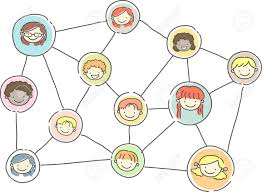
\includegraphics[width=5cm]{people_network}};

\node[anchor=north,text width=8cm] at (P.south)
{For example, the above is a representation of a network of 12 people with arcs between pairs of people who are friends.};
\end{tikzpicture}}
\end{minipage}

\begin{dingautolist}{192} 
\contentsitem{ball}{Basic network game}%
\quad\dotfill\quad\code{network_basic.py}

Our starting version of the game consists of 10 dots (or nodes using network terminology) appearing at random positions on the screen and the player has to click on the dots in correct order. As the player clicks on the dots, lines (or arcs in network terminology) are created to show progress. If the player misses or clicks on a wrong dot the path created is removed and the player has to restart.

The steps given here come from the excellent \href{https://www.dk.com/uk/book/9780241317792-computer-coding-python-games-for-kids/}{\em Coding Games with Python} book.

\contentsitem{rectangle}{Adding sounds}%
\quad\dotfill\quad\code{network_sound.py}

Go to \href{https://www.zapsplat.com}{www.zapsplat.com}, and find some sounds that we can use\\ when you click on the correct dot and when you click on an incorrect dot, and when you finish the sequence.  You could do this at home and in the coderdojo session we will show you how to convert music formats to suit pgzero.

\hfill\raisebox{-12pt}[0pt][0pt]{\href{https://www.zapsplat.com}{
\includegraphics[height=30pt]{zap-splat-logo}}}

\vspace{-12pt}

\parbox[t]{11cm}{For background music have a look at 
\href{https://www.melodyloops.com/music/}{www.melodyloops.com}\\
This has a good selection of tracks and can cut a track to whatever length you want --- you could set the length to match the time given to complete the level.}
\hfill\raisebox{-18pt}[0pt][0pt]{\href{https://www.melodyloops.com/music/}{{
\includegraphics[height=20pt]{melodyloops}}}}


\contentsitem{rectangle}{Refactor game}%
\quad\dotfill\quad\code{network_refactored.py}

Again, before we move on it is good to see how we can impove our code.

\contentsitem{rectangle}{More advanced games}%

Here we look at three ways we can build a full game from our starting network game idea.

\end{dingautolist}

%: PAGES
\renewcommand{\baselinestretch}{0.55} 


\newcommand\PAIR[3]{
\begin{landscape}\thispagestyle{empty}\hspace{-1.25cm}
\begin{tikzpicture}
\useasboundingbox (0,0) rectangle (28.1,16.75);

\ifnum#1=0\else
\node[anchor=south west] at (0,0) (L) {\includegraphics[page=#1, scale=0.707,angle=0]{\SRC}};\fi
\ifnum#2=0\else
	\node[anchor=south west] at (L.south east) (R)
	{\includegraphics[page=#2,scale=0.707,angle=0]{\SRC}};
	\fi

\node at ($(L.north east)+(0,0.5)$) {\ding{192} \color{section}\bfseries network\_basic};
#3
\end{tikzpicture}
\end{landscape}}

\def\GRID#1{
\draw (#1.south west) grid (#1.north east);
\foreach \x in {0,1,...,13} {
	\node at ($(#1.south west) + (\x,0.5) $) {\scriptsize\x}; 
	\node at ($(#1.south west) + (\x,8.5) $) {\scriptsize\x}; 
	\node at ($(#1.south west) + (\x,16.5) $) {\scriptsize\x}; 
}
\foreach \y in {1,...,16} {
	\node at ($(#1.south west) + (0, \y) $) {\scriptsize\y}; 
	\node at ($(#1.south west) + (13, \y) $) {\scriptsize\y}; 
}}


\tikzstyle{textfix}=[fill=white,anchor=south west,inner sep=0pt,outer sep=0pt,font=\textfixFont]
\tikzstyle{NWtextfix}=[textfix,anchor=north west]

\def\BUTTON#1{\includegraphics[width=12pt]{#1}}

%: PAIR 
\PAIR{72}{73}{

}


%: PAIR{74}{75}
\PAIR{74}{75}{

%\GRID{L}\GRID{R}

% step 1

\node[NWtextfix,fill=white, text width=6.4 cm] at 
	($(R.south west) + (1.7, 13.5)$) {{\bf\smaller[2] Set it up}\\[6pt]
	As usual we are going to create a separate folder to hold our network based games.\\[6pt]
	
	$\bullet$ Open your file explorer.\\[6pt]
	$\bullet$ Change directory to your {\ttfamily\smaller coderdojo\_tramore}.\\[6pt]
	$\bullet$ Inside folder  {\ttfamily\smaller coderdojo\_tramore}, create a new subfolder called  {\ttfamily\smaller network\_games}.\\[12pt]\mbox{}
};


% step 2

\node[NWtextfix,fill=white, text width=6cm] at 
	($(R.south west) + (1.7, 9.2)$) {Save your file in the folder {\ttfamily\smaller network\_games}. This should be inside your folder {\ttfamily\smaller coderdojo\_tramore}. If you have difficulty finding this folder, please ask.};

\node[textfix,fill=white] at 
	($(R.south west) + (2.7, 6.6)$) {\smaller network\_games\quad\quad\mbox{}};
\node[textfix,fill=white] at 
	($(R.south west) + (2.4,7.5)$) {\smaller network\_basic.py};

% step 3
\node[NWtextfix,fill=white,text width=5cm, text depth=3cm] at 
	($(R.south west) + (7.7,8.5)$) {};
\node[NWtextfix,fill=white,text width=4.3cm, text depth=3cm] at 
	($(R.south west) + (8.45,8.95)$)  {You can create this folder using your 
	file explorer or just by clicking on the images button \BUTTON{images} in your Mu editor.};

% step 4

\node[textfix,bottom color=gray!25,top color=gray!10] at 
	($(R.south west) + (3.3, 2.65)$) {\smaller network\_games\quad\quad\mbox{}};
\node[NWtextfix,bottom color=gray!20,top color=gray!20] at 
	($(R.south west) + (1.65,2.475)$) {\smaller network\_basic.py};


\node[postit,anchor=north west, text width=6cm] at ($(R.south west) + (1.65,1.475)$)
	{Remember, I have put a copy of the Resource Pack in 
		folder {\tt coderdojo\_trammore\backslash resources}};
	
%: step 3
\node[NWtextfix,fill=white] at 
	($(R.south west) + (10.1,4)$) {\ Mu \ };

}

%: PAIR{76}{77}
\PAIR{76}{77}{
}


%: PAIR{78}{79}
%\renewcommand{\baselinestretch}{0.55} 
\PAIR{78}{79}{

%�\GRID{L}\GRID{R}

 %: step 11
\node[NWtextfix,fill=white,text width=10cm,text depth=2cm] at 
	($(L.south west) + (1.65,15.4)$) {{\bf\smaller[3]Test Your Code}\\[3pt]
	Let's test the code that you have written so far.\\[6pt]
	Remember, it is always a good idea to check code as often as possible both to see if what you have just implemented is correct and that you have not broken some earlier code by your most recent changes.
	};

}



%: PAIR{76}{77}
\PAIR{80}{81}{
}

\clearpage

\section{Refactor game}

\TODO{Create a new file and copy the contents of \code{network_basic.py} into it. Save new file as \code{network_refactored.py} in your \code{network_games} folder. Then make the following changes.}

\begin{tikzpicture}
\tikzstyle{link}=[line width=4pt,-latex,blue]

% 

\node[text width=17cm] at (0,0) (A1)
	{\codeonly{}{10}{13}{\MUcode}{network_basic.py}};

\node[text width=16.5cm] at (1,-5.5) (B1)
	{\codeonly{}{10}{13}{\MUcode}{network_refactored.py}};

\draw[link] (A1.200) to[out=270] node (L1){}  (B1);

\node[postit,text width=15cm] at (0,-2.5) (T1) {It is important to think carefully about the names we give to our data in our programs. Here \code{dot} is better because it is more specific and more informative than \code{actor}.\\[6pt]
\todoSymbol\ \ Change identifier name from \code{actor} to \code{dot} };


% 

\node[text width=16cm] at (0,-11) (A2)
	{\codeonly{}{16}{26}{\MUcode}{network_basic.py}};

\node[text width=15cm] at (2,-17) (B2)
	{\codeonly{}{16}{26}{\MUcode}{network_refactored.py}};

\draw[link] (A2.205) to[out=270,in=180] node (L2){}  (B2);

\node[postit,text width=15cm,anchor=north west] at ($(B2.south west) +(-2,0)$) (T1) 
{In function \code{draw} I have made two changes:
\\[6pt]$\bullet\ $ 
used \code{enumerate} to count over the dots, so don't need variable \code{number} and 
\code{enumerate} will be responsible for remembering to update \code{n} and not me! But note that \code{enumerate} starts counting at zero.
\\[6pt]$\bullet\ $
the identifier \code{line} is a list of two points, rather than referring to the two points by number, it is nicer and clearer to give them names --- I have used \code{start} and \code{end}.
\\[6pt]
\todoSymbol\ \ Make the above changes.};
\end{tikzpicture}

\enlargethispage{1cm}

\clearpage
\section{More advanced games}

\subsection{Count to 50}

\TODO{Copy the contents of \code{network_refactored.py} into a new file and save it as \code{count_to_50.py} in the \code{network_games} folder.}

We can improve the current game in a number of ways --- one way is to develop the following `Count to 50' game:\\[12pt]
\begin{minipage}{12cm}
\begin{itemize}
\item
Screen starts with three (level 3) dots, and with each level the number of dots increase by one.
\item
To help the player the dots are coloured as follows: dots already joined together are blue, the next dot to click on is green, and all other dots are red.
\item
Players have 3 lives, they lose a life every time they click on an incorrect dot.
\item
The game is timed and players have to race through the levels before the time runs out. 
\end{itemize}
\end{minipage}
\hfill
\begin{minipage}{6cm}\centering
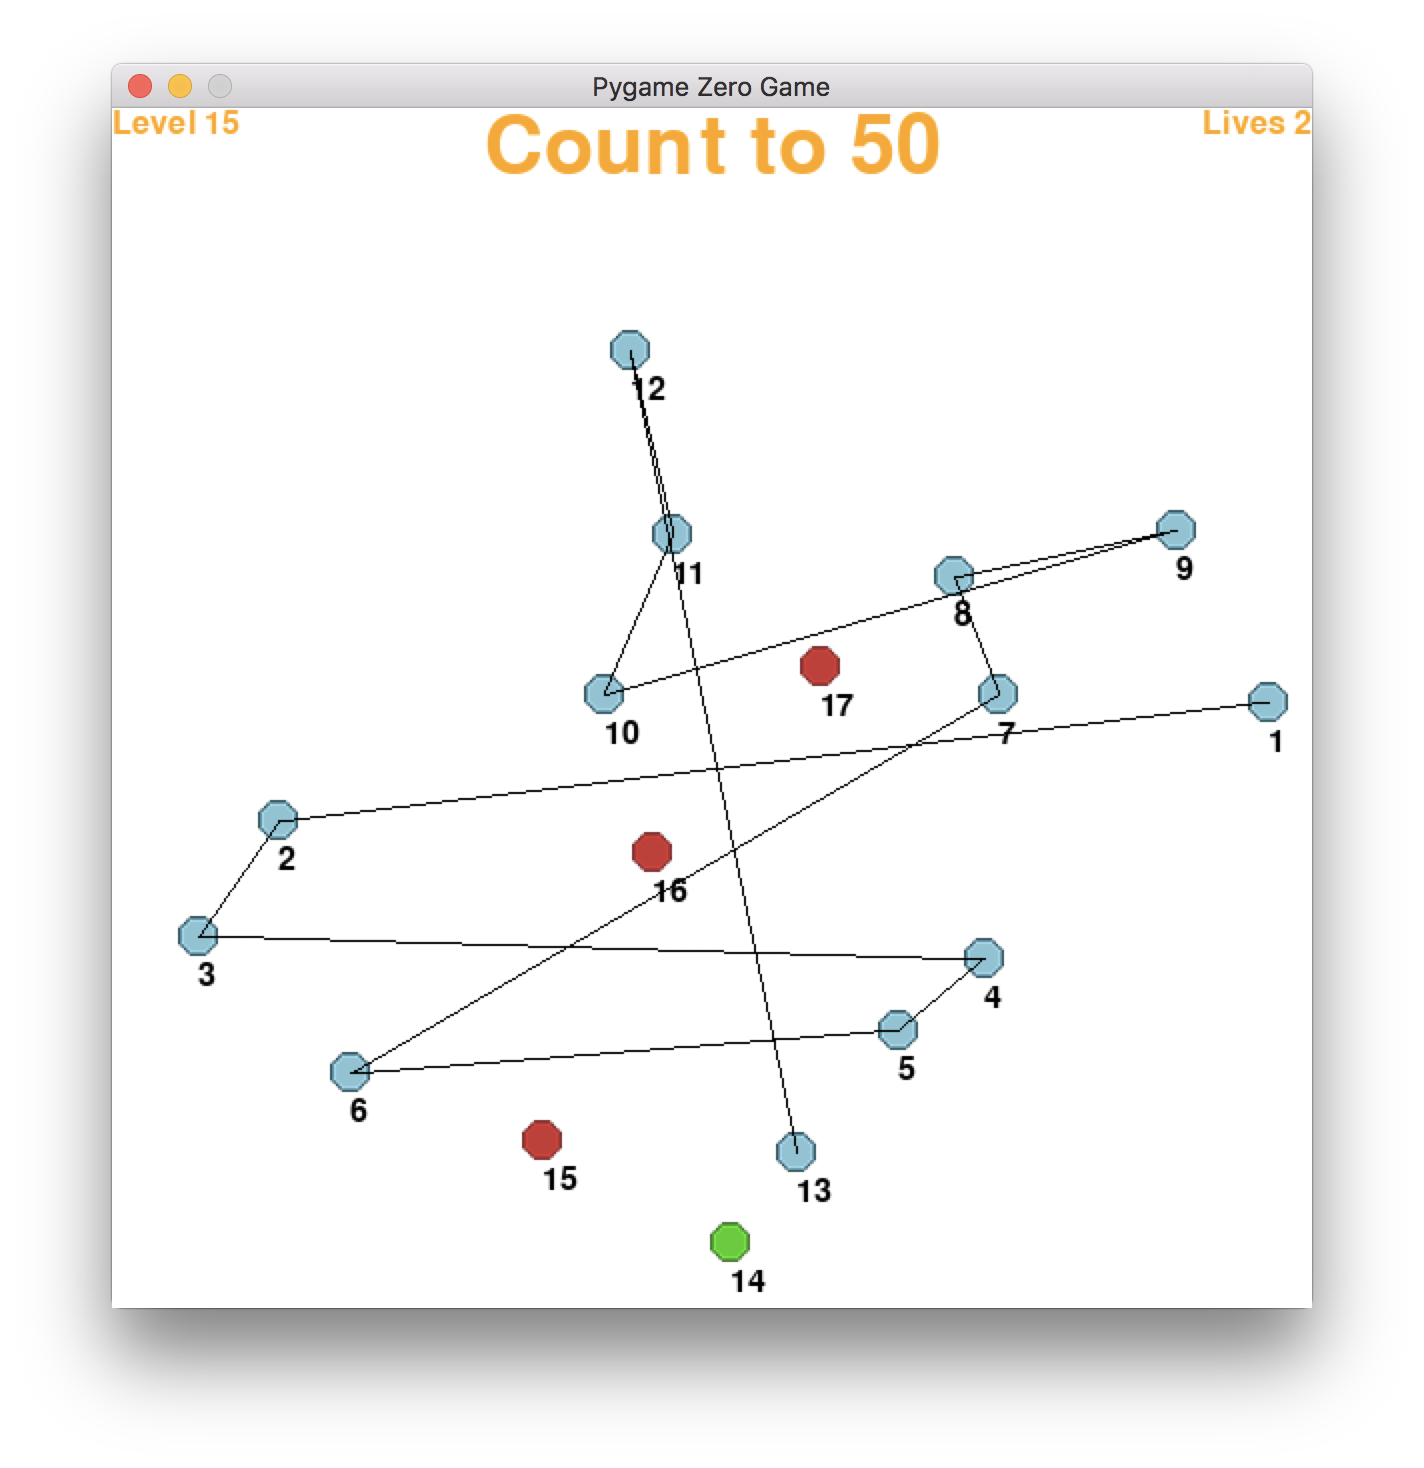
\includegraphics[width=.9\textwidth]{Count_to_50}
\end{minipage}

\begin{itemize}
\item Doing all of the levels from 3 to 50 will require a lot of clicks (will require 5044 clicks!) so we want some way for players to "hyper-jump" a few levels occasionally or gain time bonus by say getting to a dot particularly quickly. Have a think about what you could do here and talk to us in terms of how to implement your ideas.
\item One small detail remains --- when you currently generate the random positions for the dots 
sometimes one dot is (partially) covered by another. We don't want that since then the player cannot click on the correct dot.  There is an easy fix for that, but rather than us telling you, have a think about it first.
\end{itemize}

\subsection{Make a Total}

\TODO{Copy the contents of \code{network_refactored.py} into a new file and save it as \code{make_a_total.py} in the \code{network_games} folder.}

\vspace{-12pt}
% Here is a different variant of the game:
\begin{itemize}
\item Instead of counting up what about displaying at random number and the player then needs to click on dots to together sum up to the displayed figure --- they get extra points for using the fewest number of dots.  
\item 
In this version all of the dots will be blue as the player will need to decide which numbers that want to use to make the required total. If the dots clicked on go above the total then the level restarts and they lose a life,
\item
Again, to add pressure, have the levels timed so you lose a life if you don't get the total within the given time limit.
\item
One of the change that I would do to make writing this game easier is to store in each dot its label, using something like the following:

\centerline{\code{dot.label = n}}

\item Or what about going {\em extreme total} and have both green and red dots --- to get a total you add the green dots and subtract the red?  That will make life much harder!
\end{itemize}

%\subsection{Make a Total Extreme}
%
%\TODO{Copy the contents of \code{make_a_total.py} into a new file and save it as \code{make_a_total_extreme.py} in the \code{network_games} folder.}
%
%\vspace{-12pt}
%%Here is harder version of the total game:
%\begin{itemize}
%\item Instead of having one colour dots where the label values are all added together, have two colours --- where the blue dots are added but the green dots are subtracted. 
%\end{itemize}
\enlargethispage{1cm}

\end{document}